\chapter{Introduction}
\section{Brief Historical Note}
Robotics, the field of study and development of robots, has a rich and fascinating history that spans several centuries. From ancient myths and legends to the modern-day robots that have become integral parts of our lives, the evolution of robotics has been a testament to human ingenuity and technological advancements.

The concept of artificial beings can be traced back to ancient times. In Greek mythology, there are tales of Hephaestus, the god of fire and craftsmanship, who created mechanical servants to assist him in his workshop. Similarly, the Jewish folklore speaks of the Golem, a creature made of clay brought to life through mystical means. While these are more mythical in nature, they laid the foundation for the idea of creating artificial beings.

The first known attempts at building mechanical beings can be found in ancient China and Greece. In China, during the 3rd century BCE, a mechanical engineer named Yan Shi is said to have built a human-like automaton that could perform various tasks. In Greece, the mathematician and engineer Heron of Alexandria created a series of automated devices known as "automatons," including a singing bird and a self-opening temple door.

The Industrial Revolution of the 18th and 19th centuries marked a significant turning point in the development of robotics. With the advent of mass production and mechanisation, the need for automated systems became evident. In 1738, Jacques de Vaucanson, a French inventor, constructed a mechanical duck that could flap its wings, eat, and digest food, showcasing a high level of sophistication for its time.

The term "robot" itself was coined by Czech writer Karel Čapek in his play "R.U.R." (Rossum's Universal Robots) in 1920. The play depicted artificial human-like creatures, known as robots, who rebel against their human creators. This popularized the term and gave rise to the popular perception of robots as intelligent and autonomous beings.

In subsequent decades, significant advancements were made in robotics. In the 1970s, researchers began working on mobile robots capable of navigating and interacting with their environment. The 1990s saw the emergence of humanoid robots like Honda's ASIMO, which showcased remarkable dexterity and mobility. The field of artificial intelligence (AI) also played a crucial role in enabling robots to exhibit intelligent behaviors and adaptability.

Robots have found applications in various industries, including manufacturing, healthcare, agriculture, space exploration, and entertainment. They have become indispensable tools in industries where precision, efficiency, and repetitive tasks are required. Additionally, robots have also been employed in hazardous environments, such as deep-sea exploration or defusing bombs, to protect human lives.
\begin{figure}[H]
    \centering
    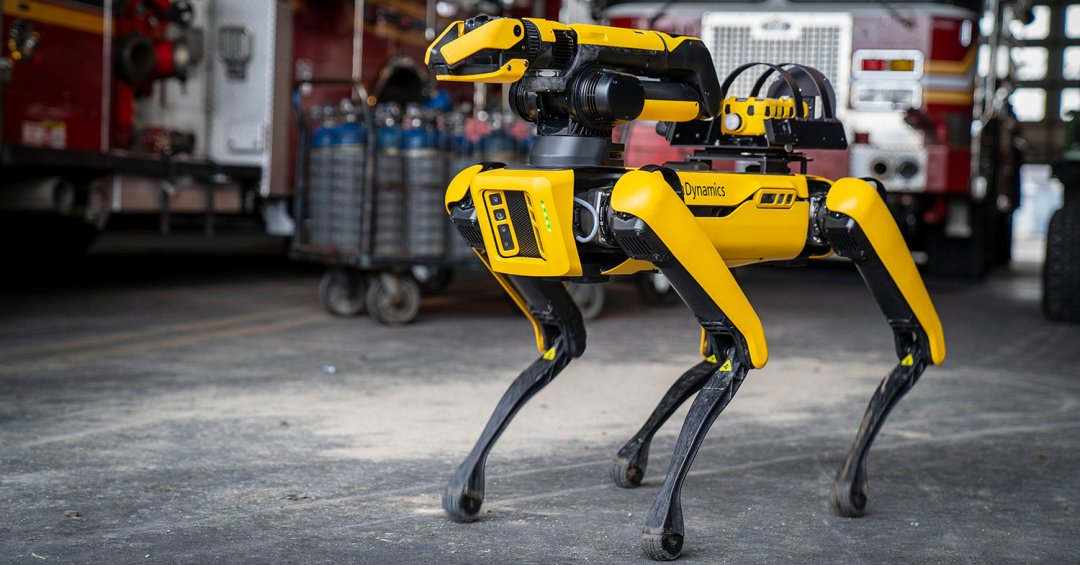
\includegraphics[scale=.45]{images/boston-dynamics-spot}
    \caption[Boston dynamics robot (spot)]{Spot an agile mobile robot from Boston dynamics. \textit{Boston dynamics is an American robotics design comapny.} (Source: IoT Today website. \cite{iotworldtoday})}
\end{figure}

In recent years, robotics has witnessed breakthroughs in areas such as machine learning, computer vision, and natural language processing. These advancements have led to the development of advanced humanoid robots, autonomous vehicles, and intelligent personal assistants.


However, the rapid advancement of robotics also raises ethical and societal concerns. The potential impact on employment, privacy, and security are areas of ongoing debate. As robots become more autonomous and capable of making decisions, questions about accountability and the boundaries of their actions arise.

Looking to the future, robotics holds immense promise. Continued advancements in AI, materials science, and sensor technology are expected to pave the way for even more sophisticated robots capable of complex tasks, improved human-robot interaction, and advancements in healthcare, space exploration, and other fields.

n conclusion, the history of robotics is a testament to human curiosity, innovation, and the desire to create artificial beings. From ancient tales to modern marvels, robotics has come a long way and continues to shape the way we live and work. As we move forward, it is essential to navigate the challenges and opportunities that arise to ensure that robotics benefits humanity as a whole.

\section{Applications of Robotics}
Robotics has a wide range of use cases in various industries and fields. Some of the most common use cases of robotics are:
\begin{enumerate}
    \item Manufacturing: Robotics is widely used in manufacturing industries for automation of production processes. Robots are used for tasks such as assembling, welding, painting, and quality inspection. The use of robotics in manufacturing has led to increased productivity, accuracy, and efficiency.

          \begin{figure}[H]
              \centering
              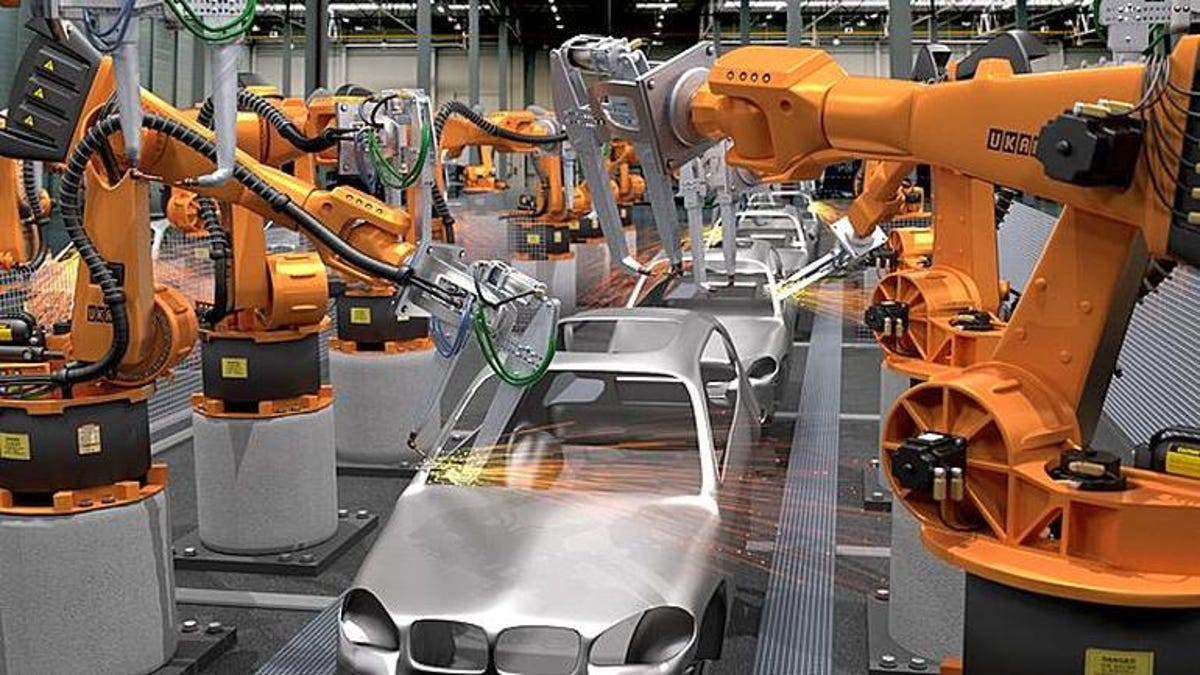
\includegraphics[scale=.225]{images/industral-robos.jpg}
              \caption[Car assembling robots]{Robots being used for car assembling (Image Source: Finance monthly.com. Url: \url{https://www.finance-monthly.com/2021/10/a-look-at-how-robots-are-used-in-the-automotive-industry/} \cite{financemonthly})}
          \end{figure}

    \item Healthcare: Robotics has been used in healthcare for various purposes, such as surgery, rehabilitation, and medication management. Robotic surgery is now commonly used for procedures such as prostatectomies, hysterectomies, and cardiac surgeries. Robotic exoskeletons are also used for rehabilitation of patients with mobility issues.

          \begin{figure}[H]
              \centering
              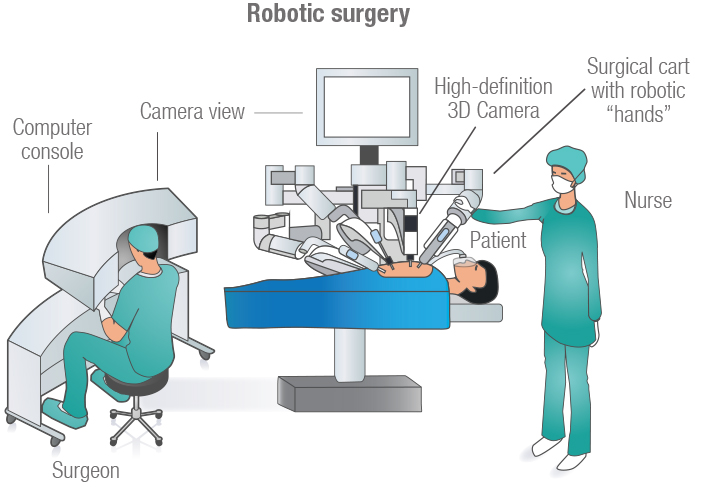
\includegraphics[scale=.5]{images/robotic-surgery-illustration}
              \caption[Robotic surgery schematic diagram]{Schematic representation of Robotic Surgery an important application of Robotics in Medicine. (Image Source: Master Private Network Website (Url: \url{https://www.materprivate.ie/our-services/robotic-surgery}))}
          \end{figure}

    \item Agriculture: Robotics has the potential to revolutionize the agriculture industry by automating tasks such as planting, harvesting, and crop monitoring. Drones are used for crop surveillance and mapping, while robotic tractors are used for planting and harvesting.

    \item Education: Robotics is used in education to teach students about programming, electronics, and mechanics. Robotics kits are used in classrooms to teach students how to build and program robots.

          \begin{figure}[H]
              \centering
              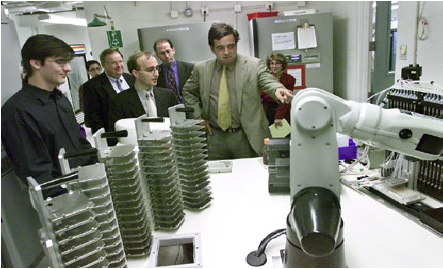
\includegraphics[scale=1]{images/robo-lab}
              \caption[Robot used in Biology and Chemistry lab]{Robot used in Biology and Chemistry Laboratory. (Image Source: \url{https://www2.lbl.gov/Publications/Currents/Archive/May-05-2000.html})}
          \end{figure}

    \item Military and Defense: Robotics is used in the military and defense industries for tasks such as bomb disposal, surveillance, and reconnaissance. Unmanned aerial vehicles (UAVs), also known as drones, are used for reconnaissance and surveillance.

    \item Space exploration: Robotics has played a critical role in space exploration, with robots being used to explore other planets and moons. NASA's Mars rovers, for example, have been instrumental in collecting data and conducting experiments on the red planet.



    \item Entertainment: Robotics is also used in the entertainment industry, such as animatronics in theme parks and movie special effects.
\end{enumerate}

\section{The Problem of Motion Planning}

Motion planning, also known as path planning or trajectory planning, is a fundamental problem in robotics and artificial intelligence. It involves determining a feasible path or trajectory for a robot or agent to navigate from a starting point to a goal location while avoiding obstacles and respecting constraints.

The significance of motion planning lies in its crucial role in enabling autonomous robots to operate effectively and safely in real-world environments. By solving the motion planning problem, robots can navigate complex and dynamic environments, accomplish tasks efficiently, and interact with the world in a meaningful way. Here are some key aspects highlighting the significance of motion planning:

\begin{enumerate}
    \item \textbf{Collision Avoidance:} One of the primary objectives of motion planning is to ensure collision-free movements for robots. Robots often operate in environments where there are obstacles or other dynamic entities, such as humans. Motion planning algorithms help robots avoid collisions by generating paths or trajectories that navigate around obstacles or safely interact with the environment.
    \item \textbf{Efficiency and Optimal Resource Utilisation:} Motion planning algorithms aim to find paths or trajectories that optimize various objectives, such as minimizing travel time, energy consumption, or wear and tear on the robot's components. Efficient motion planning algorithms enable robots to move swiftly and accomplish tasks in the most optimal manner, leading to improved productivity and resource utilisation.
    \item \textbf{Task Execution:} Motion planning is closely tied to task execution for robots. By efficiently planning robot motions, tasks can be executed smoothly and in a coordinated manner. This is particularly important in applications such as industrial automation, where robots need to perform precise and synchronized actions in manufacturing processes.
    \item \textbf{Adaptability and Robustness:} Motion planning algorithms need to account for dynamic environments and unforeseen changes. They must be able to handle uncertainties, such as moving obstacles, changes in the environment, or sensor errors. Robust motion planning techniques allow robots to adapt and replan their paths in real-time, ensuring the safe and efficient completion of tasks even in dynamic scenarios.
    \item \textbf{Human-Robot Interaction:} As robots become more integrated into our daily lives, it is crucial to develop motion planning algorithms that enable safe and intuitive human-robot interactions. Robots should be able to navigate and move in a way that is comfortable and predictable for humans, respecting social norms and ensuring safety.
    \item \textbf{Multi-Robot Systems:} Motion planning becomes even more challenging in scenarios involving multiple robots that need to coordinate their actions. Cooperative motion planning algorithms enable multiple robots to collaborate, share information, and optimize their paths to achieve collective objectives efficiently. This is relevant in applications such as warehouse automation, swarm robotics, and search and rescue missions.
    \item \textbf{Safety and Risk Mitigation:} Motion planning plays a crucial role in ensuring the safety of robots and their interactions with humans. By considering safety constraints and incorporating risk assessment, motion planning algorithms can avoid potentially dangerous situations and minimize the risk of accidents or collisions.
\end{enumerate}

In summary, motion planning is a critical problem in robotics with broad implications. It allows robots to navigate complex environments, avoid collisions, optimize resource utilisation, execute tasks efficiently, adapt to changing conditions, interact safely with humans, and coordinate actions in multi-robot systems. Solving the motion planning problem is essential for the advancement and widespread adoption of autonomous robots in various domains, ranging from manufacturing and healthcare to transportation and home assistance.

However, developing the technologies necessary for autonomous robots is a formidable undertaking with deep interweaved ramifications in automated reasoning, control and perceprion, which raises many important problems, one of them which is \textbf{motion planning}, which is the major theme of this project work. Since we live in a dynamic and unpredictable environment it is not possible to explicitly describe all the possible motions that a robot may have to exeecute in order to accomplish a requested task. Hence the need for algorithms

This work focus on the topological study of robot motion planning algorithms using results from algebraic topology and some other important areas of mathematics, and we also give the implementation of the RRT algorithm using the C++ programming language.

%%%%TODO add the references to each of the mentioned works
\section{Literature Review}
Motion planning is a fundamental problem in robotics. It is the problem of finding a safe and efficient path for a robot to move from one point to another in its environment. The environment may be cluttered with obstacles, and the robot may have limited mobility. Motion planning is a challenging problem, and there is no single algorithm that can solve all cases.

The topology of robot motion planning is an important topic in robotics research, as it involves the study of the configuration space and its topology, which is crucial for path planning and obstacle avoidance. A literature review on this topic reveals that researchers have explored various approaches to tackle the challenges associated with robot motion planning, such as high dimensionality, non-convexity, and dynamic environments.

One common approach is to use sampling-based methods, such as the Probabilistic Roadmap (PRM) and Rapidly-exploring Random Trees (RRT). These methods rely on sampling the configuration space to build a roadmap or tree structure that represents the connectivity of the space, allowing for efficient path planning. However, the topology of the configuration space can still pose challenges, particularly in the presence of narrow passages or high-dimensional spaces.

To address these challenges, researchers have proposed various techniques that leverage the topology of the configuration space. For example, the Topological Roadmap (TRM) method constructs a graph that represents the topology of the configuration space by identifying critical points and their connectivity, allowing for efficient path planning even in higher-dimensional space. Similarly, the Topological RRT (TRRT) method incorporates topology into the RRT algorithm by using a tree structure that preserves the topology of the configuration space.

An algebraic approach to the problem of motion planning was introduced in 1983 by Schwartz and Sharir ~\cite{schwartz:1983a} where they presented an algorithm for solving the two-dimensional case of the problem, using the \textit{Piano movers problem} as a motivation. In 1988, John Canny studied the complexity of motion planning algorithms which is the study of the time taken for a given algorithm to move a robot from one configuration to another ~\cite{canny1988}.

The sampling-based approach was introduced in the work of Steven LaVelle, where he introduced the Rapidly-Exploring Random Tree (RRT) algorithm. Modifications were made to optimize the RRT algorithm with the development of the RRT* algorithm by Michael Montemerlo. To date, many other algorithms (such as A*, Theta, Theta*, etc) have been introduced to improve the existing algorithms.

The topological approach to robot motion planning was introduced in 2003-2004 by Michael Farber. His motivation was using tools from algebraic topology, whereby he considered a path-connected topological space whose path space is equipped with the compact open topology. By this, the motion planning algorithm of any mechanical robot that moves in a configuration space is represented by the function of input and output with the input being the two points (that is the current location of the robot and its destination) and the output is the path to be taken by the robot.

In the earlier work by Farber, he introduced a homotopy invariant called Topological complexity, which measures the minimum number of continuous motions required to move a robot from one configuration to another in a given configuration space \cite{farber2003topological}. In this founding paper, he was only concerned with the departing motion of the robot and not the returning motion, but made up for this in a subsequent work in 2007 \cite{farber2007symmetric} where the concept \textit{symmetric topological complexity} was introduced and it was used to studied the case when the departing and returning motion of the robot are the same.

Using the motivation of Farber and Grant, in 2015 Derfoufi and Mamouni considered the case when the robot is allowed to take any arbitrary path to come back to its departure point, as in the case of the motion of drones, or an unmanned aeroplane, or a guided TV camera, they studied homotopically and topologically the concept of \textit{loop motion planning algorithm (LMPA)}  and define the \textit{loop topological complexity} which is a generalisation of the work of Farber and Grant \cite{derfoufi2015loop}. In the same spirit Rami  studied another variant of topological complexity for bundled fibre space in 2018 \cite{rami2018variant}.

In 2016, Derfoufi and Mamouni used the F\'elix-Thomas generalisation of the Chas-Sullivan \textit{String topology} into rational homotopy to generalize \textit{string topology} into a broad topological robotics settings and research continues on that.

In 2018, Pavesic used the topological complexity of Farber to study the degree of instability of the manipulation plan for a mechanical device describing its kinematic maps \cite{pavesic2018topologist}.

A very recent work by Farber, Cohen and Weinberger studied the parametrized motion planning algorithms, where they introduced the parametrized topology complexity and studied the collision-free motion of multiple robots in a 3-dimensional space \cite{cohen2021topology}.


